\documentclass{llncs}
\usepackage{amsmath,amssymb,amsfonts}
\usepackage{algorithmic}
\usepackage{graphicx}
\usepackage{textcomp}
\usepackage{xcolor}
\usepackage{booktabs}
\usepackage{multirow}
%\usepackage{acrodef}
\usepackage[printonlyused]{acronym}
\usepackage{float}
\usepackage{orcidlink}
\usepackage{placeins}
\acrodef{HRC}{Human-Robot Collaboration}
\acrodef{EEG}{Electroencephalography}
\acrodef{EMG}{Electromyography}
\acrodef{EDA}{Electrodermal Activity}
\acrodef{ECG}{Electrocardiography}
\acrodef{AI}{Artificial Intelligence}
\acrodef{XGBoost}{eXtreme Gradient Boosting}
\acrodef{MLP}{Multilayer Perceptron}
\acrodef{ATTR}{Automatic Task-Type Recognition}

\begin{document}

\title{Task Recognition from Physiological Data Using Multimodal Sensor Fusion For Human-Robot Collaboration}

\author{Ameur Gargouri\inst{1}\orcidlink{0009-0001-8293-037X} \and Mohamed Karray\inst{2}\orcidlink{0000-0001-7293-8696} \and Mohamed Ksantini\inst{3}\orcidlink{0000-0002-9928-8643}}

\institute{ESME Research Lab \\
    ATISP Laboratory, ENET'Com\\
    University of Sfax\\
    Ivry-sur-Seine, France / Sfax, Tunisia\\
    \email{ameur.gargouri.doc@enetcom.usf.tn}
    \and
    ESME Research Lab\\
    Ivry-sur-Seine, France\\
    \email{mohamed.karray@esme.fr}
    \and
    ATISP Laboratory, ENET'Com\\
    University of Sfax\\
    Sfax, Tunisia\\
    \email{mohamed.ksantini@ipeis.usf.tn}}
\maketitle

\begin{abstract}
    Automatic task-type recognition from operator physiological data is a key capability for adaptive assistive human-robot collaboration. Assistance can be adapted in real time when a robot can detect an operator's current task state from physiological signals quickly and reliably. This requires a preprocessing path that behaves identically across algorithms, a fusion scheme that combines heterogeneous sensor groups without letting one group dominate, and an explicit account of what the resulting labels do and do not represent. We propose a compact multimodal pipeline that standardizes preprocessing, fuses sensor-derived features into a unified tabular representation, and trains detectors with class-aware objectives. The pipeline is applied to MultiPhysio-HRC dataset. Every protocol condition is mapped to exactly one of five task conditions, namely cognitive load, high stress, industrial task, low load, and other, by a deterministic rule that we release in full. %We audit the feature export before modelling and remove 16 recording-identifier columns and 96 duplicated \ac{EEG} columns that would otherwise leak recording identity and double-weight the \ac{EEG} block, leaving 128 features. 
    Results show that \ac{XGBoost} achieves the best performance with 0.9512 accuracy and 0.9104 macro-F1. A modality ablation confirms that fusion is justified rather than assumed: the fused input improves macro-F1 over the better single modality for every detector tested, by 0.047 to 0.186. We also report the scope of these figures candidly, since the hold-out shares operators between its splits, and we measure inference latency to assess real-time feasibility.
    \keywords{physiological signals, task recognition, multimodal fusion, human-robot collaboration, assistive systems}
\end{abstract}

\section{Introduction}
\Ac{HRC} is a form of shared control in which a human operator and a robot coordinate actions in real time to accomplish a task safely, efficiently, and transparently \cite{selvaggio2021autonomy,borghi2025operatorstress}. The robot must continuously interpret the operator's state and adjust its behavior as the interaction evolves. To achieve this, a training phase must be accomplished, based on data collected from sensors related to the operator and the robot. In this work, we treat only data from the operator physiological signals. Human-side data include physiological and behavioral cues such as \ac{EEG}, \ac{EMG}, \ac{EDA}, \ac{ECG}, respiration, and related measurements that can reveal human intentions, obtained from a multimodal dataset by construction.

Different sensors provide complementary information, but weak fusion can overfit subject-specific artifacts or fail to capture the relationships between modalities. Moreover, the target task labels are often imbalanced and may not be perfectly separable from the current representation, which can lead to overfitting and unreliable predictions.

This paper presents an applied system for task-condition recognition built on the MultiPhysio-HRC multimodal dataset, which contains five task conditions: cognitive load, high stress, industrial task, low load, and other \cite{bussolan2025multiphysiohrc}. We build a compact multimodal fusion pipeline that maps heterogeneous physiological signals to a single tabular representation, compare five detectors under one shared protocol, and test whether fusing modalities is justified rather than assuming it. The models are evaluated on a stratified 80/20 train-test split, and we report the resulting baselines together with their scope so that they can be used in assistive \ac{HRC} applications.

%\subsection*{Contributions}
%This paper makes four contributions. We define a deterministic and reproducible five-class task-condition schema for the \mbox{MultiPhysio-HRC} dataset, in which all 21 protocol conditions are mapped to classes by a rule that depends only on the recorded condition name, with the rule and the per-condition window counts released in full and with no crowdsourcing or subjective rating involved. We then audit the feature export before any modelling so that the reported figures rest on physiological features rather than on the acquisition pipeline's own bookkeeping, which leaves a 128-feature representation. On that representation we run a controlled comparison of five detectors under one shared protocol, and we add a modality ablation for this dataset that tests the fused input against the better single modality per detector and shows that fusion helps in every case, which addresses a gap we identified in prior work where fusion is assumed rather than tested. We close with a candid statement of evaluation scope, since the reported figures are a within-subject ceiling rather than an across-operator estimate, and we quantify the direction of that difference and measure inference latency so that the deployment claims are bounded by measurement.

%\subsection*{Organization}
Section~\ref{sec:related} reviews related work on physiological task recognition and multimodal fusion in \ac{HRC}. Section~\ref{sec:method} describes the proposed methodology, covering the pipeline, the data and the label schema, the problem formulation, detector selection, the training process, and the metrics. Section~\ref{sec:results} presents the benchmark, the modality ablation, the class-level analysis, and the latency measurements, and Section~\ref{sec:conclusion} concludes.

\section{Related Work}
\label{sec:related}

Physiological operator-state recognition for \ac{HRC} has advanced through new datasets, new fusion models, and new evaluation studies. This section outlines recent contributions in each of these areas and identifies the drawback that motivates the present work.

Bussolan et al.~\cite{bussolan2025multiphysiohrc} introduced the MultiPhysio-\ac{HRC} dataset used in this paper and reported recognition of self-reported stress and cognitive-load levels on an industrial assembly task, reaching macro-F1 ranges of roughly 0.34--0.39 for stress and 0.33--0.49 for cognitive load across conditions \cite{bussolan2024stressdetector}. Those targets come from questionnaire instruments that are not part of the public feature export, and the source study neither audits its feature export for leakage nor tests whether fusing modalities helps under a controlled design. Our work uses the same dataset but a different, protocol-derived target, and adds both the audit and the fusion test.

Borghi et al.~\cite{borghi2025operatorstress} assessed operator stress in collaborative robotics with a multimodal approach and reported large variance across individuals. Aygun et al.~\cite{aygun2022assistive} estimated cognitive workload for assistive robots from physiological signals and likewise observed pronounced between-subject variability. These works establish that the operator effect is a central difficulty, but they evaluate single-target states on single-architecture pipelines, so the relative contribution of features, fusion, and evaluation design remains entangled.

On the fusion side, Baltrusaitis et al.~\cite{baltrusaitis2019multimodal} provide the standard taxonomy of multimodal machine learning, arguing that heterogeneous streams carry complementary information and that naive fusion can hurt when modalities are redundant or noisy. Recent work has begun to pair fusion with explicit subject-independent design, as in Cheng et al.~\cite{cheng2025crosssubject}, who fuse \ac{EEG} with eye-tracking for cross-subject cognitive-load recognition and combine a cross-attention fusion mechanism with domain-adversarial adaptation so that the learned representation transfers to unseen participants. That combination is promising, but it still assumes rather than tests the value of fusion itself. The taxonomy of Baltrusaitis et al.\ remains largely descriptive, and controlled empirical tests on physiological \ac{HRC} data, where redundancy across channels is high, remain scarce. Our modality ablation is a step toward filling that gap.

On the evaluation side, Iarlori et al.~\cite{iarlori2024cognitiveworkload} survey cognitive-workload estimation from wearable sensors in human-machine interaction and catalogue the evaluation heterogeneity that makes studies hard to compare. Jin et al.~\cite{jin2025cognitivestate} provide a recent systematic review of physiological cognitive-state recognition and show that the design of the data split is among the largest drivers of reported performance differences. That concern has since been quantified: Brookshire et al.~\cite{brookshire2024leakage} contrast segment-based and subject-based holdouts on \ac{EEG} and find that the segment-based protocol strongly overestimates performance on new subjects, and their survey of the literature shows that most translational deep-learning studies use exactly that protocol. Reviews of the workload literature reach a parallel conclusion from the task side, where Pu\v{s}ica et al.~\cite{pusica2025workload} report a significant drop in classification accuracy when workload is induced by multitasking and rated by quantitative task load rather than subjectively, and Diarra et al.~\cite{diarra2025realworld} note that the metrics used in controlled laboratory studies rarely transfer to real-world settings. These reviews identify the problem but do not supply a concrete recipe for the compact applied setting we target.

Finally, Selvaggio et al.~\cite{selvaggio2021autonomy} survey autonomy levels in physical human-robot interaction and identify reliability, transparency, and adaptation as the constraints that any state estimator must serve. Task-state recognition is a building block of such autonomy, and our latency and failure-mode discussion speaks to the deployment requirements they enumerate.

Recent work points toward several responses to the difficulties above. Bussolan et al.~\cite{bussolan2025federated} extend the same line of multimodal operator monitoring with federated learning, training on-device over \ac{EEG}, \ac{ECG}, \ac{EDA}, \ac{EMG}, and respiration so that stress prediction is personalized without moving raw signals off the operator's equipment. Wei et al.~\cite{wei2025sgatcn} address the task-dependence of workload signatures instead, using a stacked graph attention convolutional network that reaches 0.651 accuracy when the model must generalize across N-back, mental arithmetic, and Sternberg tasks, which shows how much accuracy is lost once the task itself no longer identifies the label. At the representation level, Jiang et al.~\cite{jiang2024labram} pretrain a large \ac{EEG} model on roughly 2{,}500 hours drawn from about 20 datasets and fine-tune it across clinical and affective tasks, which shows that generic \ac{EEG} representations are now feasible. None of these lines, however, reports a compact audited pipeline on a single public \ac{HRC} dataset that separates the contribution of the features from the contribution of fusion, which is the gap we address.

In summary, prior work establishes that fusion of physiological modalities is promising in principle \cite{baltrusaitis2019multimodal,cheng2025crosssubject}, that operator-state recognition in \ac{HRC} is hard and subject-dependent, and that evaluation design determines reported performance. What is missing is a compact and reproducible account of task-condition recognition on a public \ac{HRC} dataset that audits the features before modelling, states the label rule exactly, and tests whether fusion helps. The present work addresses that gap.

\section{Methodology}
\label{sec:method}

\subsection{Proposed Solution Pipeline}

The proposed solution follows the pipeline summarized in Figure~\ref{fig:pipeline}. Physiological signals are first cleaned and normalized through the preprocessing stage, then transformed into a unified tabular fused representation. Alongside that fused representation we retain two modality feature groups, one holding the \ac{EEG} channels and one holding the peripheral channels, because the ablation of Section~\ref{sec:ablation} reuses the identical preprocessing path on each group separately. The three representations are passed to the selected detector models, which ensures a consistent input structure and therefore makes any difference in outcome attributable to the detector rather than to the data preparation.

The preprocessing stage carries more weight than its name suggests, because the export it consumes is not yet a clean feature matrix. That export is a table of 257 columns in which physiological summaries sit beside the acquisition pipeline's own bookkeeping, namely operator and repetition identifiers, dataset flags, and duplicate copies of columns that already exist. Removing that bookkeeping belongs to the method itself rather than to housekeeping, since a model trained on it learns the recording instead of the task and counts some evidence twice, and a pipeline that skips this step cannot separate what the model learned about the task from what it learned about the recording. Section~\ref{sec:prep} states the audit in full, and every detector reported below is trained on the 128 features that survive it.

The fusion step itself operates as follows. The \ac{EEG} block contributes 96 features, that is, 12 statistical summaries computed over each of 8 channels. The peripheral block contributes 32 features, that is, 8 summaries over each of 4 signal families, namely \ac{ECG}, \ac{EDA}, \ac{EMG}, and respiration. Concatenating the two blocks yields the 128-dimensional fused vector that every tabular detector consumes. For the two-tower neural model the two blocks are not concatenated at the input. Each block is instead projected by its own tower into a compact embedding, and only the two embeddings are concatenated before the prediction head. This design lets the network learn a separate representation per modality group before mixing them, which is the structural difference between the two-tower model and the tabular detectors that receive the same 128 features as one flat vector.

\begin{figure}[H]
    \centering
    
\includegraphics[width=\columnwidth]{task_pipeline.png}
    \caption{Proposed pipeline, from preprocessing to the shared evaluation protocol.}
    \label{fig:pipeline}
\end{figure}

\subsection{Data and Preprocessing}
\label{sec:prep}

Reliable deployment of the proposed detector requires one consistent preprocessing path across algorithms. The main training data source is MultiPhysio-HRC, a multimodal industrial \ac{HRC} dataset combining physiological and behavioral measurements across controlled and realistic collaborative tasks \cite{bussolan2025multiphysiohrc}. We therefore apply one fixed sequence of operations to every input configuration. Metadata and non-feature columns are removed first, after which all candidate features are coerced to numeric values and columns that are null throughout the export are discarded. Task labels are then mapped into the unified five-class schema of Table~\ref{tab:labels}. Missing values are filled by median imputation, the features are standardized using training-fold statistics only, and the result is assembled into the unified tabular fused representation together with the per-modality feature groups that the ablation of Section~\ref{sec:ablation} reuses.

The column audit deserves a precise statement, because the export we obtained is wider than the physiological measurement it is supposed to contain. Of its 257 columns only 128 hold a genuine physiological feature, and the remaining 129 are bookkeeping of four different kinds that must be separated rather than treated alike. 16 columns carry recording identifiers and trial counters, among them columns prefixed \texttt{ID\_\_} and \texttt{Repetition\_\_}, which record which operator and which repetition produced the row. 8 further columns are dataset metadata and presence flags, which describe the export rather than the person. Neither of these two families measures anything about the operator.

An identifier column is a documented route by which a classifier learns to recognize the recording rather than the condition \cite{brookshire2024leakage}. The mechanism is worth stating plainly, because within a single recording the operator identity is nearly constant while the class label changes. A model that can read the identifier can therefore memorize which operator produced a window and score well on held-out windows from that same operator without having learned anything about the task, which is why an identifier inflates a random split while telling nothing about a new operator. We drop these 24 columns, and with them 24 opportunities to memorize the recording.

96 further columns are byte-identical duplicates, meaning that each one repeats the exact numerical values of an existing \ac{EEG} feature column under a different name. They add no information, but they are not harmless either. A model that weighs columns as evidence now receives the \ac{EEG} block twice, so the duplication would silently give \ac{EEG} a weight of 192 columns against 32 peripheral columns, and any comparison between modalities would be settled by the bookkeeping rather than by the signal. We drop these 96 columns as well, which brings the number of removed columns to 120.

The remaining nine columns are identifier and label keys. Unlike the columns above they are not deleted, because the split and the scoring still need to know which window belongs to which class. They are held aside and are never passed to a detector as inputs. What the detectors see is therefore the 128 genuine features, distributed as 96 \ac{EEG}, 8 \ac{ECG}, 8 \ac{EDA}, 8 \ac{EMG}, and 8 respiration features, which is 257 minus the 120 removed columns and the 9 keys. The retained set contains 328 missing values in total, which median imputation fills using training-fold statistics only.

\subsection{Task-Condition Labels}

The dataset annotates each recording with the protocol condition that was performed. We therefore define the recognition target as the task condition, which the experimental protocol itself certifies. Each window receives exactly one of five labels, assigned deterministically from the recording's condition name by the rule released with the reproducibility package. Because the labels are a deterministic function of the protocol, they are exact and reproducible, and there is no ambiguity about which condition a window came from.

The five classes are defined by the protocol conditions that produce them, rather than by an abstract psychological interpretation. Table~\ref{tab:labels} gives the complete mapping for all 21 conditions together with the resulting window counts.

\begin{table}[!h]
    \caption{Deterministic mapping from the 21 protocol conditions to the five classes.}
    \label{tab:labels}
    \centering
    \footnotesize
    \begin{tabular}{@{}llr@{}}
        \toprule
        Class           & Protocol conditions, \texttt{task\_name}                                                               & Windows \\
        \midrule
        cognitive load  & \texttt{stroopeasy\_0}, \texttt{stroophard\_0}, \texttt{n-back\_0}, \texttt{hanoi\_0}, \texttt{mat\_0} & 975     \\
        high stress     & \texttt{vr-plank\_0}                                                                                   & 224     \\
        industrial task & \texttt{manual-task-1}\dots\texttt{-5}, \texttt{cobot-task-1}\dots\texttt{-5}                          & 3{,}571 \\
        low load        & \texttt{rest-1}, \texttt{rest-2}, \texttt{rest\_0}, \texttt{meditation\_0}                             & 799     \\
        other           & \texttt{vr-job-sim\_0}                                                                                 & 71      \\
        \midrule
        Total           & 21 conditions                                                                                          & 5{,}640 \\
        \bottomrule
    \end{tabular}
\end{table}


The mapping is coherent with a physiological hypothesis in each case. The cognitive-load conditions, namely the Stroop battery in its easy and hard variants, the N-back task, the Tower of Hanoi, and an arithmetic and puzzle task, tax working memory and executive control. The high-stress condition is a virtual-reality height-plank walking task, a validated stressor that induces threat-related autonomic arousal. The industrial-task conditions are ten physical assembly and order-picking blocks, five performed manually and five with a collaborative robot, which mix physical and cognitive demands in realistic \ac{HRC} settings. The low-load conditions are rest and guided-meditation segments between the demanding blocks and provide a low-demand baseline. The residual class holds a single open-ended virtual-reality job-simulation session that belongs to none of the controlled batteries. We keep it as its own class rather than forcing it into another, and we report its small size explicitly.

The class distribution is strongly imbalanced, with 3{,}571 windows for industrial task against 224 for high stress and 71 for other. In proportional terms the majority class accounts for 63.3 percent of the data, high stress for 4.0 percent, and other for 1.3 percent. A classifier that always predicts industrial task therefore reaches 0.633 accuracy while recovering none of the minority states, which is why accuracy alone cannot rank models on this dataset and why the metrics of Section~\ref{sec:metrics} and the class weights of Section~\ref{sec:formulation} are necessary.

\subsection{Problem Formulation}
\label{sec:formulation}

Physiological task recognition in this work is formulated as a supervised five-class classification problem on multimodal sensor-derived representations. Let $z_i$ denote the synchronized measurements acquired from the operator, that is, the \ac{EEG}, \ac{EMG}, \ac{EDA}, \ac{ECG}, and respiration channels, over an observation interval. After preprocessing and fusion, each interval is mapped to a tabular feature vector $x_i \in \mathbb{R}^{d}$ with $d = 128$, and carries a label $y_i \in \{1,\ldots,5\}$ drawn from the five task conditions in the order cognitive load, high stress, industrial task, low load, and other.

Given a model $f_\theta$ with parameters $\theta$, the class posterior for class $c$ on input $x_i$ is written $p_\theta(y=c\mid x_i)$. To handle the class imbalance documented above, training minimizes a class-weighted cross-entropy objective:
\begin{equation}
    \mathcal{L}(\theta)= -\frac{1}{N}\sum_{i=1}^{N}\sum_{c=1}^{5} w_c\,\mathbf{1}[y_i=c] \log p_\theta(y=c\mid x_i),
    \label{eq:loss}
\end{equation}
where $N$ is the number of training windows, $c$ indexes the five classes, $\mathbf{1}[\cdot]$ is the indicator function, and $w_c$ is the weight assigned to class $c$. The predicted label is obtained by
\begin{equation}
    \hat{y}_i = \arg\max_{c\in\{1,\ldots,5\}} p_\theta(y=c\mid x_i).
    \label{eq:pred}
\end{equation}

The weight $w_c$ is the part of Eq.~\eqref{eq:loss} that responds to the measured imbalance. We set $w_c = N / (5 N_c)$ and then rescale the vector so that its mean is one, where $N_c$ is the number of training windows of class $c$. With equal class sizes this reduces to uniform weighting. On the observed distribution it assigns the majority class a weight of about 0.32 and the smallest class a weight of about 16, which is what prevents the objective from being minimized by a model that simply reproduces the majority class. The word \emph{class-aware} is used throughout to mean exactly this weighting scheme.

\subsection{Algorithm Selection}
We focus on a pragmatic set of models that are practical for deployment on fused tabular features: logistic regression, random forest, \ac{XGBoost} \cite{chen2016xgboost}, \ac{MLP}, and a compact two-tower fusion architecture. The two-tower model explicitly separates modality groups, as described in Section~\ref{sec:method}. This design emphasizes an operational fusion pattern that is compact and suitable for integration in assistive systems. %The four tabular detectors are implemented with scikit-learn \cite{pedregosa2011scikit}.

\subsection{Training Process}
The training process is designed to be simple, transparent, and reproducible across algorithms: we create a stratified 80/20 train-test split with a fixed random seed of 42, fit preprocessing only on training data, and then apply the same transforms to held-out data. For neural models, optimization uses Adam with class-weighted cross-entropy and early stopping under the same fixed seed, where the early-stopping slice is itself stratified so that it observes every class. For classical models, class balancing is applied through model-specific weighting when supported.
This unified protocol ensures that performance differences mainly reflect model behavior rather than inconsistent data handling. The hyperparameter settings are listed in Table~\ref{tab:hyper}.

\begin{table}[!h]
    \caption{Detector hyperparameters on the shared 128-dimensional representation.}
    \label{tab:hyper}
    \centering
    \small
    \begin{tabular}{@{}lp{9.25cm}@{}}
        \toprule
        Model               & Configuration                                                                                                                       \\
        \midrule
        Logistic Regression & L2 penalty, \texttt{max\_iter} 2000, balanced class weights                                                                         \\
        Random Forest       & 300 trees, balanced class weights                                                                                                   \\
        \ac{XGBoost}        & 400 estimators, depth 6, learning rate 0.05, subsample 0.9, column subsample 0.9                                                    \\
        \ac{MLP}            & hidden layers 128 and 64, Adam, \texttt{max\_iter} 600                                                                              \\
        Two-Tower Fusion    & per-modality towers 128 then 64, head 64 then 5, dropout 0.2, Adam at 1e-3, weight decay 1e-4, batch 256, early-stopping patience 8 \\
        \bottomrule
    \end{tabular}
\end{table}

\subsection{Metrics and Diagnostics}
\label{sec:metrics}
For this five-class physiological dataset, metric choice is tied to the observed class imbalance and to the operational need for reliable performance across all task states \cite{sokolova2009systematic}. We report accuracy as a global indicator of overall correct decisions, but we do not rely on it alone, because as Section~\ref{sec:method} shows, the majority class alone already accounts for 0.633 accuracy, and accuracy is known to overstate performance under this degree of imbalance \cite{jeni2013imbalanced}. We therefore report balanced accuracy, which averages recall across classes and better reflects sensitivity to minority states such as low load and other \cite{brodersen2010balanced}. We also report macro-F1 as the primary ranking metric because it jointly penalizes low precision and low recall at the class level while weighting all classes equally.

To complement scalar scores, we analyze row-normalized confusion matrices and per-class precision, recall, and F1 for the selected detector. These diagnostics identify which task pairs are confused and verify whether strong aggregate performance is maintained across individual classes under the same stratified 80/20 hold-out protocol.

% \subsection{Reproducibility}
% \label{sec:repro}
% The reported pipeline is fully specified by the following quantities. The dataset contributes 52 operators, 21 protocol conditions, and 5{,}640 analysis windows. Each window is 60 seconds long with 50 percent overlap between consecutive windows, and each feature is a statistical summary computed within the window. No window is discarded, so the analyzed count equals the exported count. The cleaned feature matrix has shape 5{,}640 by 128 and contains 328 missing values. The split is stratified by class with a test fraction of 0.2, giving 4{,}512 training windows and 1{,}128 test windows. Missing values are imputed with training-fold medians, and standardization uses training-fold statistics. The random seed is 42 throughout, and no hyperparameter search was performed on the test set, so the reported figures are single-configuration results rather than the outcome of tuning. Software versions are scikit-learn 1.7.2, XGBoost 3.3.0, PyTorch 2.12.1, pandas 2.3.3, and NumPy 2.3.5.

% The code that produces every number in this paper, the deterministic label rule, the feature manifest recording which columns were kept and which were dropped, and the derived result tables are released together as a reproducibility package so that the pipeline can be rerun end to end.

\section{Results and Discussion}
\label{sec:results}

\subsection{Comparison}

We compare the proposed detector against the selected baselines under the stratified 80/20 hold-out and identify the strongest operating point for the fused physiological representation. Table~\ref{tab:results} summarizes the resulting ranking, and Figure~\ref{fig:results_detectors} shows the same comparison as grouped bars so that the three metrics can be read side by side.

\begin{table}[!h]
    \caption{Benchmark results under the stratified 80/20 hold-out, ranked by macro-F1.}
    \label{tab:results}
    \centering
    \begin{tabular}{lccc}
        \toprule
        Model               & Accuracy & Balanced Acc. & Macro-F1 \\
        \midrule
        \acs{XGBoost}       & 0.9512   & 0.8819        & 0.9104   \\
        Random Forest       & 0.9264   & 0.8350        & 0.8773   \\
        \acs{MLP}           & 0.9184   & 0.8391        & 0.8457   \\
        Two-Tower Fusion    & 0.8732   & 0.8350        & 0.8324   \\
        Logistic Regression & 0.7686   & 0.7132        & 0.6597   \\
        \bottomrule
    \end{tabular}
\end{table}

The pattern is stable across all three metrics, and the ordering has a mechanistic reading rather than being a numerical accident. Tree-based ensembles lead because the fused representation is a table of 128 marginal statistical summaries, and axis-aligned splits exploit monotone marginal effects efficiently without needing any cross-feature interaction to be modelled explicitly. \ac{XGBoost} edges out the random forest by 0.033 macro-F1 because boosting fits successive trees to the residual class confusion, which matters precisely for the minority classes that a bagged ensemble tends to under-serve. The \ac{MLP} sits slightly below the tree ensembles, which is consistent with the sample size: at 4{,}512 training windows and 128 features, a 128-by-64 network has enough parameters to overfit relative to the effective number of independent observations, and the gap of 0.065 macro-F1 is the price of that capacity. Logistic regression trails clearly at 0.6597 macro-F1 despite a much smaller gap on balanced accuracy, which is the signature of a linear decision boundary that separates the classes in aggregate but cannot carve out the minority regions.

The two-tower fusion architecture is the informative case. Its balanced accuracy of 0.8350 matches the random forest exactly, yet its macro-F1 of 0.8324 is 0.045 below it. Balanced accuracy and macro-F1 differ only in how precision enters, so the pattern indicates that the two-tower model recovers the minority classes about as often as the random forest but pays a precision penalty when it does. Explicit modality separation therefore preserves useful signal and keeps the model lightweight, but it does not by itself beat a well-tuned tree ensemble on this representation and at this sample size. We report that outcome as measured rather than framing the architecture as the best option.

\begin{figure}[H]
    \centering
    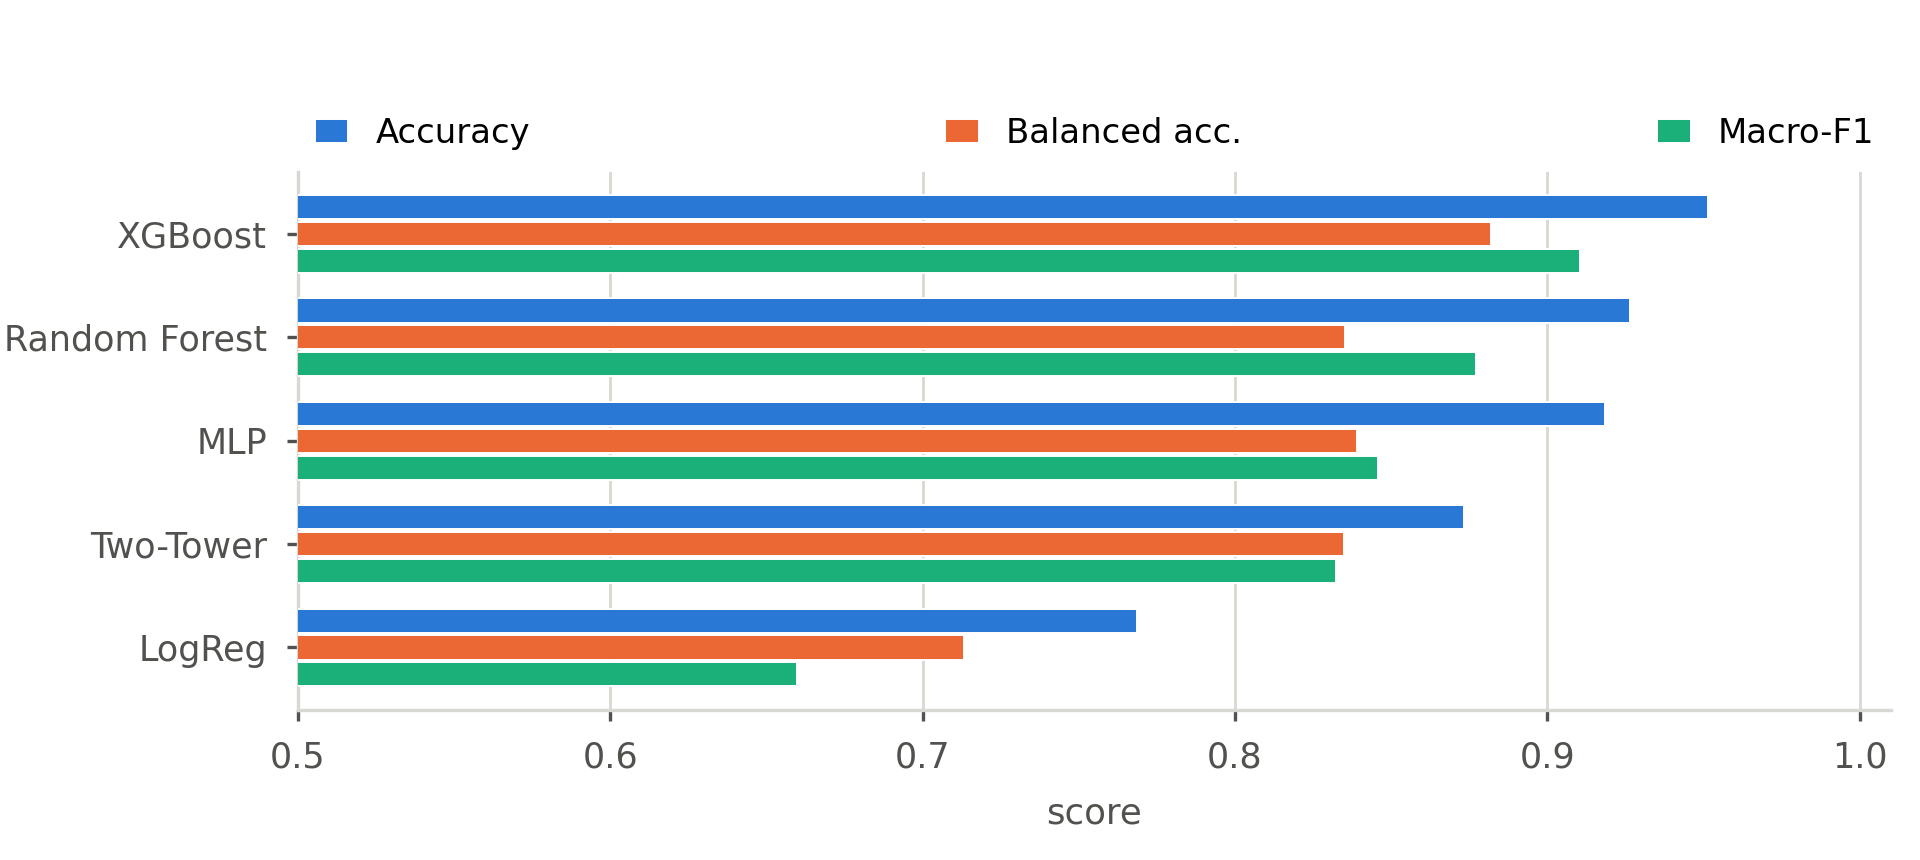
\includegraphics[width=\columnwidth]{results_detectors.png}
    \caption{Detector ranking across the three evaluation metrics.}
    \label{fig:results_detectors}
\end{figure}

\subsection{Does Fusion Help?}
\label{sec:ablation}

A ranking of detectors on the fused input does not by itself show that fusion is responsible for the performance. The fused input could be carried entirely by one modality, in which case the second modality adds cost without adding information. To test this directly, we retrain each tabular detector on three input sets under the identical split, namely \ac{EEG} only with 96 features, peripheral only with 32 features, and the fused 128 features. Table~\ref{tab:ablation} reports the outcome.

\begin{table}[!h]
    \caption{Modality ablation under the identical hold-out.}
    \label{tab:ablation}
    \centering
    \begin{tabular}{lccccc}
        \toprule
        Model               & Better single & Single & Fused & $\Delta$ & McNemar $p$ \\
        \midrule
        \acs{XGBoost}       & Peripheral    & 0.841  & 0.910 & $+0.070$ & $<10^{-4}$  \\
        Random Forest       & \ac{EEG}      & 0.784  & 0.877 & $+0.093$ & $<10^{-4}$  \\
        \acs{MLP}           & Peripheral    & 0.799  & 0.846 & $+0.047$ & $0.004$     \\
        Logistic Regression & Peripheral    & 0.475  & 0.661 & $+0.186$ & $<10^{-4}$  \\
        \bottomrule
    \end{tabular}
\end{table}

Fusion helps for every detector, and the improvement is statistically significant in all four cases after the exact McNemar test on paired per-window correctness. The result therefore answers the question rather than assuming it. The magnitude of the gain varies in an interpretable way. Logistic regression benefits most at $+0.186$, which is expected because a linear model gains the most from concatenating two views that are each only partially informative, since it cannot construct an interaction between them on its own. The tree ensembles gain less, between $+0.070$ and $+0.093$, because they can already model interactions within whichever single view they receive, so the second view contributes genuinely new information rather than recoverable structure. The \ac{MLP} gains the least at $+0.047$ with the weakest evidence, at $p = 0.004$ but the smallest effect, which is consistent with the capacity explanation given above.

A further and less obvious observation is that the better single modality is not the same for every detector. The random forest does better on \ac{EEG} alone, whereas \ac{XGBoost}, the \ac{MLP}, and logistic regression do better on the peripheral channels alone. This is worth stating because it means no single modality is uniformly dominant, and a study that tested fusion against only one of the two single-modality baselines could report a misleading conclusion in either direction. Figure~\ref{fig:results_fusion} plots the gain as a dumbbell, so that the distance between the two markers can be read directly as the size of the effect that the delta column reports.

\begin{figure}[H]
    \centering
    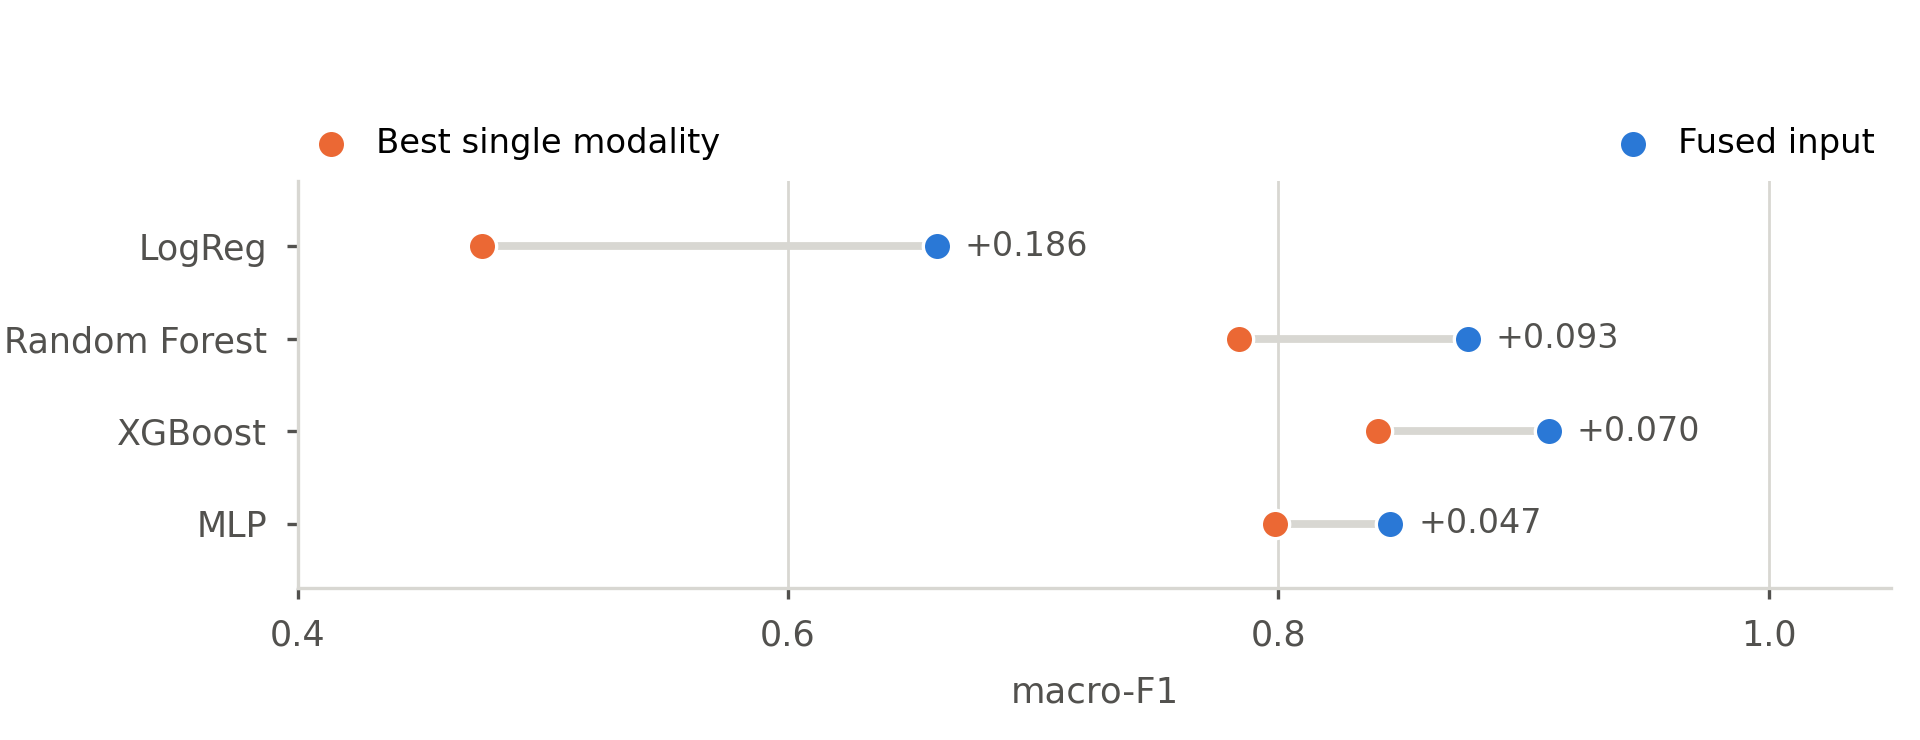
\includegraphics[width=\columnwidth]{results_fusion.png}
    \caption{Fusion gain over the best single modality for each detector.}
    \label{fig:results_fusion}
\end{figure}

\subsection{Class-Level Analysis}
\label{sec:perclass}

We inspect the selected detector at class level to understand which task states are recovered cleanly and where the remaining errors concentrate. Figure~\ref{fig:cm} shows how the selected \acs{XGBoost} model distributes its errors on the same stratified 80/20 test split, and Table~\ref{tab:perclass} provides the corresponding class-level precision, recall, and F1-score.

\begin{figure}[!ht]
    \centering
    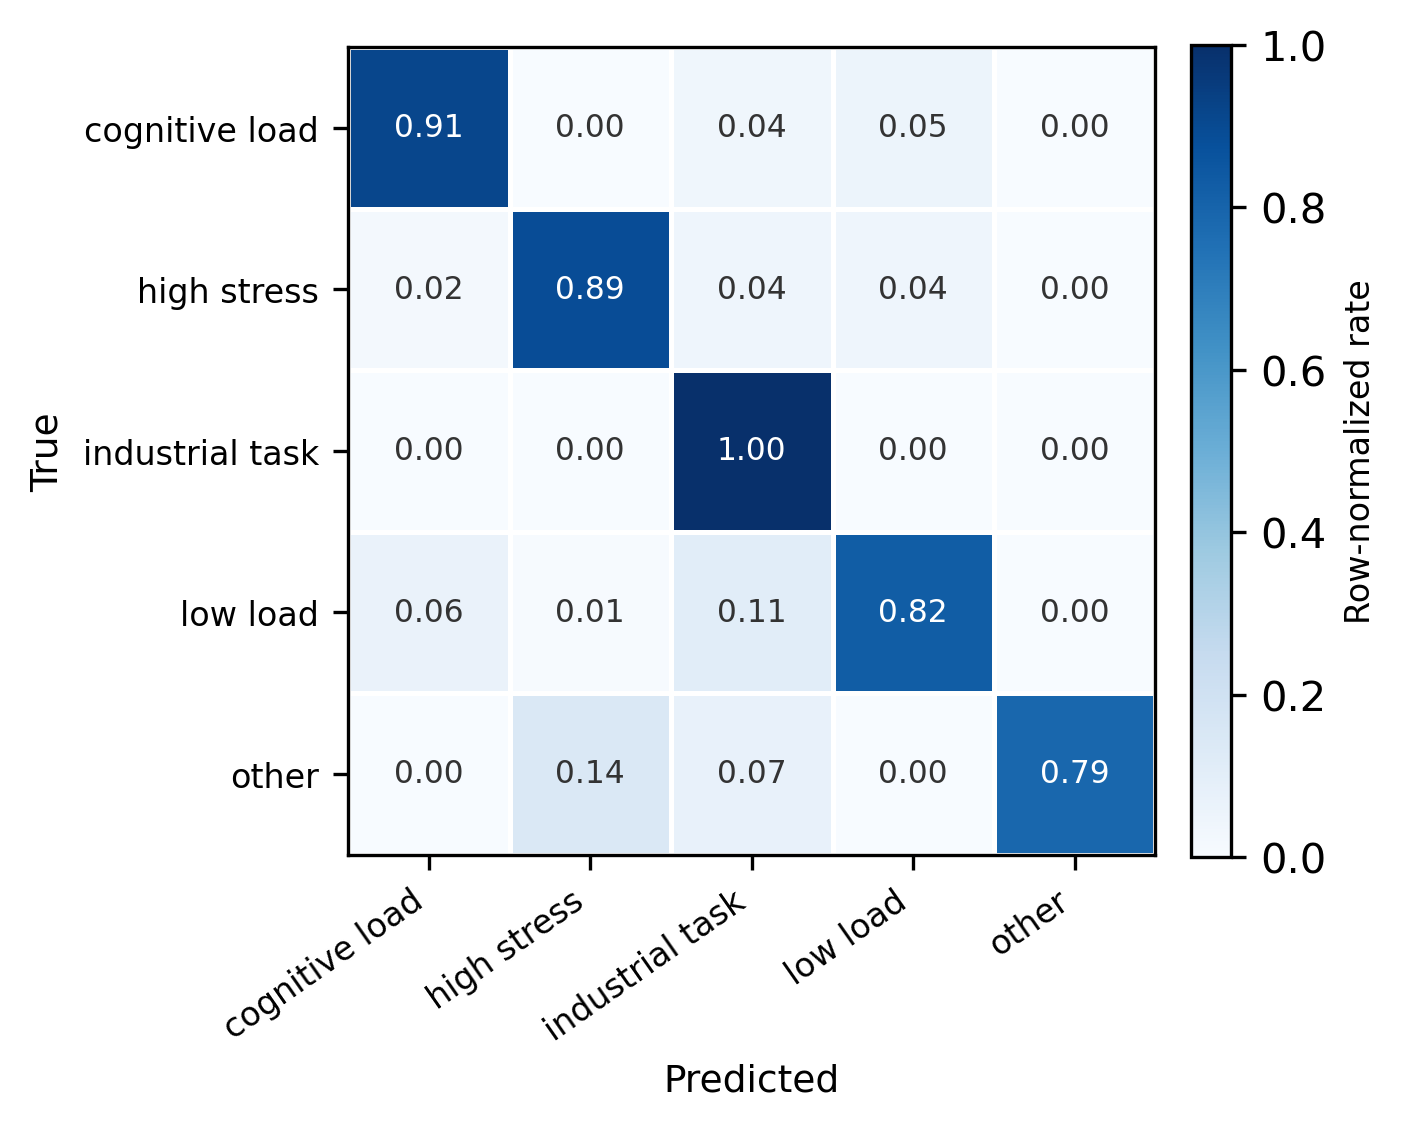
\includegraphics[width=0.68\columnwidth]{confusion_matrix_xgboost_8020_clean.png}
    \caption{Row-normalized confusion matrix for the selected \acs{XGBoost} detector.}
    \label{fig:cm}
\end{figure}

\begin{table}[!ht]
    \caption{Per-class metrics for the selected \acs{XGBoost} detector.}
    \label{tab:perclass}
    \centering
    \begin{tabular}{lrrr}
        \toprule
        Class            & Precision & Recall & F1-score \\
        \midrule
        cognitive\_load  & 0.9368    & 0.9128 & 0.9247   \\
        high\_stress     & 0.9091    & 0.8889 & 0.8989   \\
        industrial\_task & 0.9635    & 0.9972 & 0.9800   \\
        low\_load        & 0.9167    & 0.8250 & 0.8684   \\
        other            & 1.0000    & 0.7857 & 0.8800   \\
        \bottomrule
    \end{tabular}
\end{table}

The diagonal of the confusion matrix is dominant, confirming that most task states are recovered reliably, while the remaining off-diagonal mass is concentrated in a small number of confusions among semantically close states. The per-class table explains the aggregate macro-F1 reported above and clarifies the ordering in a way the scalar score cannot.

Industrial task is recovered almost perfectly, at 0.9972 recall, which is expected given that it is both the majority class and the most distinctive condition, since the assembly blocks involve sustained physical movement that the peripheral channels capture directly. Low load is the most difficult state, at 0.8250 recall, and the confusion matrix shows where its errors go: 11 percent of low-load windows are predicted as industrial task and 6 percent as cognitive load. Both directions are physically plausible, because a rest segment that immediately follows a demanding block still carries residual arousal, and the 60-second window with 50 percent overlap means adjacent windows straddle the boundary between conditions. The residual class shows the opposite profile, with perfect precision but 0.7857 recall, meaning that when the model predicts it, it is never wrong, but it misses about one window in five. That asymmetry is what a small class produces under class weighting: the weight pushes the model to be cautious about predicting a class it has seen only 71 times, so it abstains more often than it errs. High stress sits between these extremes at 0.8889 recall, confused mainly with cognitive load, which is again consistent with both conditions producing autonomic arousal.

\subsection{Real-Time Feasibility}

An assistive robot must react within the timescale of the interaction, so a detector that is accurate but slow does not answer the deployment question. Table~\ref{tab:latency} reports the median per-window inference cost of each detector on CPU, measured over repeated timed batches after warm-up, and Figure~\ref{fig:results_latency} shows the same costs on a logarithmic scale so that detectors two orders of magnitude apart stay legible side by side. Logistic regression is the cheapest at about 2.1 microseconds per window, the two-tower model follows at roughly 2.4 microseconds, the multilayer perceptron costs 4.9 microseconds, \acs{XGBoost} costs about 11 microseconds, and the random forest is the most expensive at approximately 232 microseconds, which is about 111 times the cost of the cheapest detector. The spread is therefore wide enough to matter for a deployment even though every detector is fast in absolute terms, and the cost ordering does not follow the accuracy ordering, because the cheapest model is the weakest on macro-F1 and the most expensive is only the second strongest. A deployment therefore has to trade one against the other rather than take the top of either list.

\begin{table}[H]
    \centering
    \small
    \caption{Median per-window inference cost on CPU for each detector.}
    \label{tab:latency}
    \begin{tabular}{@{}lrrr@{}}
        \toprule
        Detector            & Latency ($\mu$s) & Throughput (windows/s) \\
        \midrule
        Logistic Regression & 2.1              & 479,048                \\
        Two-Tower           & 2.4              & 412,159                \\
        MLP                 & 4.9              & 203,033                \\
        XGBoost             & 11.4             & 87,760                 \\
        Random Forest       & 232              & 4,317                  \\
        \bottomrule
    \end{tabular}
\end{table}

\begin{figure}[H]
    \centering
    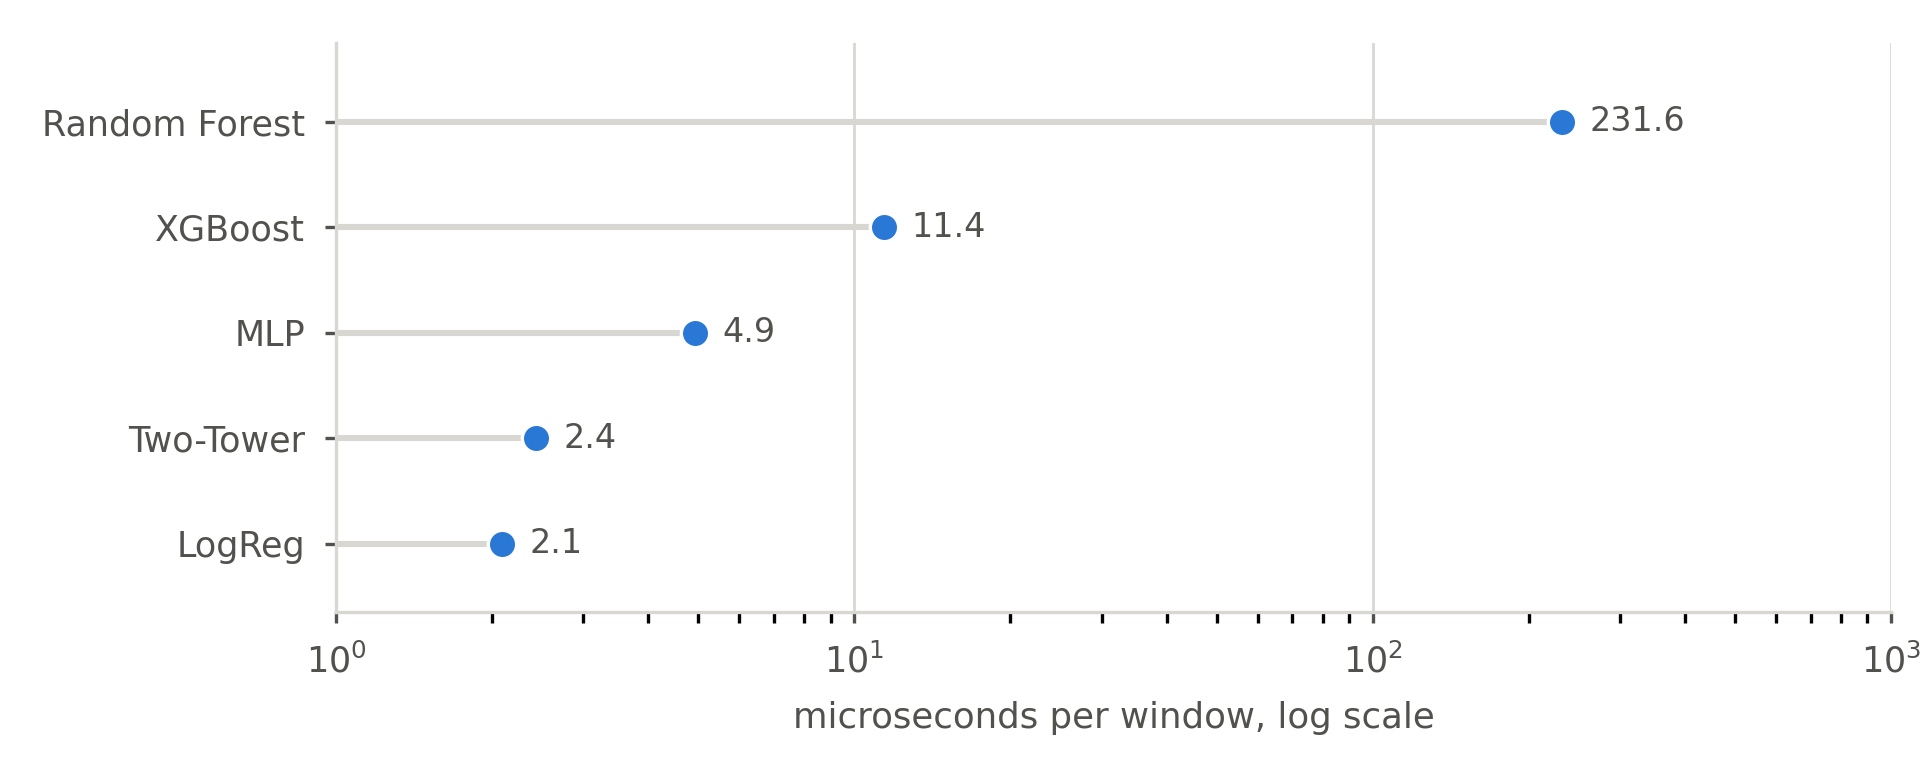
\includegraphics[width=\columnwidth]{results_latency.png}
    \caption{Median inference cost per window for each detector.}
    \label{fig:results_latency}
\end{figure}

% \section{Discussion}
% \label{sec:discussion}

% \subsection{Threats to Validity}

% The most important limitation of this study concerns the evaluation protocol. The stratified 80/20 split divides windows, not operators, so windows from the same operator appear in both the training and the test partition. Because physiological baselines are strongly operator-specific, part of the measured performance reflects the model recognizing an operator it has already seen rather than recognizing the task condition in a new person. The figures in Tables~\ref{tab:results}, \ref{tab:ablation}, and \ref{tab:perclass} should therefore be read as a within-subject ceiling, that is, as an upper bound on what this representation supports, rather than as an estimate of across-operator performance. A subject-disjoint re-evaluation of the same features, in which all windows of a held-out operator are excluded from training, yields a substantially lower macro-F1, which confirms that the operator effect is the dominant source of difficulty and that our headline numbers are optimistic in absolute terms. We report the within-subject figures because the modality ablation and the detector ranking are both computed under one identical protocol and their relative conclusions are what this paper contributes, but a reader should not transfer the absolute values to a deployment setting without an across-operator study.

% A second limitation is that the recognition target is the protocol condition rather than the operator's experienced state. The dataset also contains self-report instruments, but those are not part of the public feature export, so we cannot claim to recognize self-reported stress or workload. The five classes are behaviourally distinct and protocol-certified, which makes them reproducible, and they are not a substitute for affective ground truth.

% A third limitation is that the residual class rests on 71 windows from a single session. Its per-class figures carry wide uncertainty and should be treated as indicative. We kept it as a separate class rather than merging it precisely so that this weakness is visible rather than hidden inside another class.

% Finally, the feature audit removes the leakage we could detect, namely the recording-identifier columns and the byte-identical duplicates, but we cannot rule out subtler dependencies within the exported features, such as normalization statistics computed across the whole recording.

% \subsection{Privacy and Workplace Use}

% Physiological monitoring in a workplace raises concerns that accuracy figures do not address. Three constraints follow from the design of this system. First, the intended deployment is on-device: the pipeline consumes 128 tabular features per 60-second window and the fastest detectors run in single-digit microseconds, so inference can be performed locally without transmitting raw physiological signals off the operator's equipment. Second, the recognized target is the task condition and not the person, and the system should not be used to score, rank, or evaluate individual operators, since the evaluation above shows that operator identity is entangled with the signal and any per-person comparison would confound the two. Third, participation should be revocable: because assistance is adaptive rather than safety-critical in the conditions studied here, an operator must be able to disable the detector and fall back to a non-adaptive mode without losing robot functionality. These are design commitments rather than empirical findings, and we state them so that the scope of the contribution is clear.

\section{Conclusion}
\label{sec:conclusion}
Adaptive human-robot collaboration requires reliable recognition of the operator's task state from multimodal and user-dependent physiological signals, because downstream assistance depends on timely and accurate interpretation of the current situation. In this paper, we proposed a compact applied task-condition recognition system based on fused physiological features, class-aware learning, and a unified training pipeline for five task conditions. We defined the five classes by a deterministic rule over the 21 protocol conditions and released that rule in full, audited the feature export and removed 120 non-feature columns, and evaluated five detectors on the resulting 128-feature representation. The results show that the fused representation supports strong task discrimination, with \ac{XGBoost} providing the best operating point in our experiments at 0.9512 accuracy and 0.9104 macro-F1.

We also tested the premise of the paper rather than assuming it. A modality ablation under the identical protocol shows that the fused input improves macro-F1 over the better single modality for every detector, by between 0.047 and 0.186, and that no single modality is uniformly dominant across detectors. We further stated the scope of the reported numbers candidly: because the hold-out shares operators between its partitions, the figures are a within-subject ceiling, and a subject-disjoint evaluation of the same features gives a substantially lower result.

Future work will focus on real-life deployment and on expanding the available task varieties in the dataset. The most valuable next step is a subject-disjoint evaluation with an explicit across-operator estimate, since that is the quantity a deployment decision actually depends on, followed by assessing how the system behaves when exposed to a broader range of physiological patterns and collaborative situations.

\newpage
\bibliographystyle{splncs04}
\bibliography{task_type_detection_references}

\end{document}
